\section{Systembeschreibung im Zustandsraum}
\subsection{Allgemein (Mehrgrößensystem MIMO) }
	\begin{mdframed}[style=exercise]
		\vspace{-1em}
		\begin{align*}
			\dot{\Vec{x}}(t) & = A\vec{x}(t) + B\vec{u}(t) \quad x(0) = x_{0} \\
			\vec{y}(t)       & = C\vec{x}(t) + D\vec{u}(t)
		\end{align*}
	\end{mdframed}

	\begin{center}
		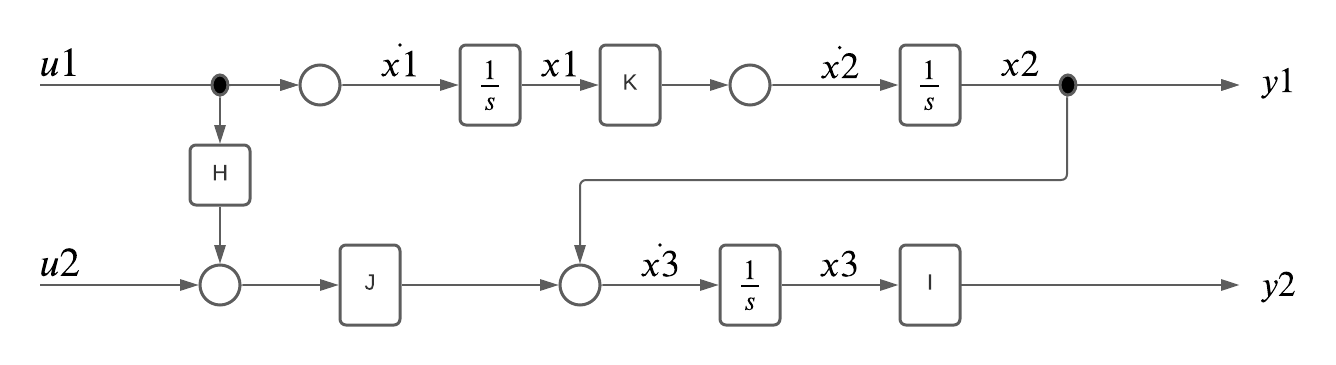
\includegraphics[width=0.96\columnwidth]{Figures/zustandsraum/Signalflussplan.png}
		\captionof{figure}{Signalflussplan}
	\end{center}

	\begin{mdframed}[style=exercise]
		\begin{align*}
			\dot{x}_{1} & = 0\cdot x_{1} +0\cdot x_{2} +0\cdot x_{3} +1\cdot u_{1}+0\cdot u_{2}        \\
			\dot{x}_{2} & = K\cdot x_{1} +0\cdot x_{2} +0\cdot x_{3} +0\cdot u_{1}+0\cdot u_{2}        \\
			\dot{x}_{3} & = 0\cdot x_{1} +0\cdot x_{2} +0\cdot x_{3} +H\cdot J\cdot u_{1}+J\cdot u_{2} \\
			\dot{y}_{1} & = 0\cdot x_{1} +1+x_{2} +0\cdot x_{3} +0\cdot u_{1}+0\cdot u_{2}             \\
			\dot{y}_{2} & = 0\cdot x_{1} +0\cdot x_{2} +l\cdot x_{3} +0\cdot u_{1}+0\cdot u_{2}        \\
		\end{align*}
	\end{mdframed}

	\begin{mdframed}[style=exercise]
		\[A = \begin{bmatrix}
				0 & 0 & 0 \\
				K & 0 & 0 \\
				0 & 0 & 0
			\end{bmatrix} \ 
			B = \begin{bmatrix}
				1         & 0 \\
				0         & 0 \\
				H\cdot{}J & J
			\end{bmatrix}\]
		\[C = \begin{bmatrix}
				0 & 1 & 0 \\
				0 & 0 & l \\
			\end{bmatrix} \
			D = \begin{bmatrix}
				0 & 0 \\
				0 & 0
			\end{bmatrix}
		\]
	\end{mdframed}

	Eigenwerte der A-Matrix liefern Pole:\\
	\begin{align*}
		\operatorname{det}(A - sI) \overset{!}{=} 0
	\end{align*}

\subsubsection{Polfestlegung durch vollständige Zustandsrückführung}

\centering
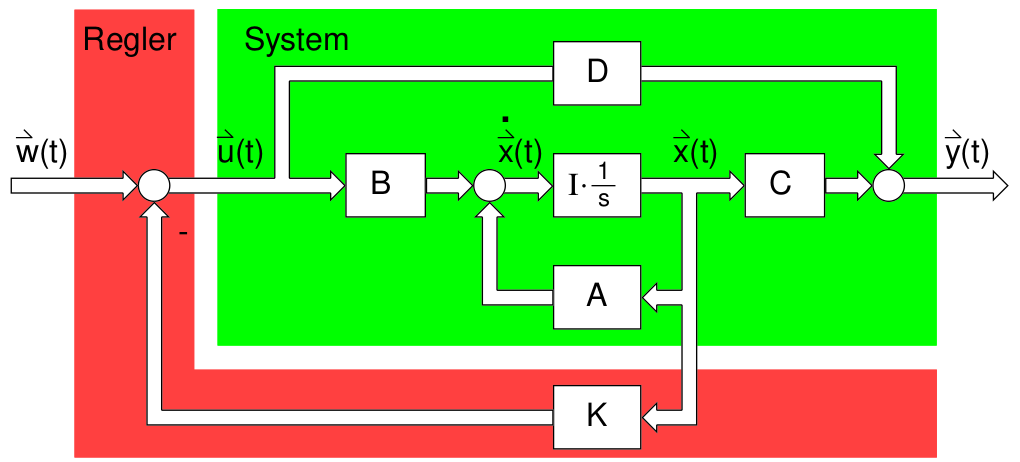
\includegraphics[width=0.8\columnwidth]{Figures/zustandsraum/Polfestlegung.png}

\raggedright
Durch die freie Wahl von K können alle n Pole des Systems beliebig platziert
werden.

Von jeder Zwischengröße \(x_i\) eine Rückführung auf jede Eingangsgröße \(u_j\) mit einem Verstärkungsfaktor \(K_{ij}\) möglich.\\
Die Rückführung führt zu einem neuen System, bei dem die Eingangsgröße \(u_j\) durch die Rückführung von \(x_i\) beeinflusst wird.\\
Zur Bestimmung der neuen Systemmatrix \(A_{RK}\) nach der Rückführung wird die Rückführungsmatrix \(K\) in die ursprüngliche Systemmatrix \(A\) integriert.

Die neue Systemmatrix \(A_{RK}\) muss die gewünschten Pole erhalten.
\begin{align*}
	&\operatorname{det}(A_{RK} - sI) \overset{!}{=} 0 \\
	\Rightarrow &\operatorname{det}(A_{RK} - sI) \overset{!}{=} \text{Nenner von } F(s)_{\text{gew\"unscht}}
\end{align*}
